\begin{figure}[t]
\centering
    \begin{subfigure}[t]{\columnwidth}
    \centering
      \caption{Ainu (left) -- Japanese (right)}
      \vspace{-0.5em}
      \fbox{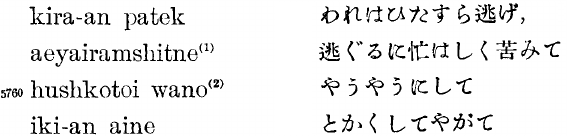
\includegraphics[width=0.9\columnwidth]{images/ainu_ex.png}}
      \vspace{0.6em}
    \end{subfigure}
    \begin{subfigure}[t]{\columnwidth}
      \centering
      \caption{Griko (top) -- Italian (bottom)}
      \vspace{-0.5em}
      \frame{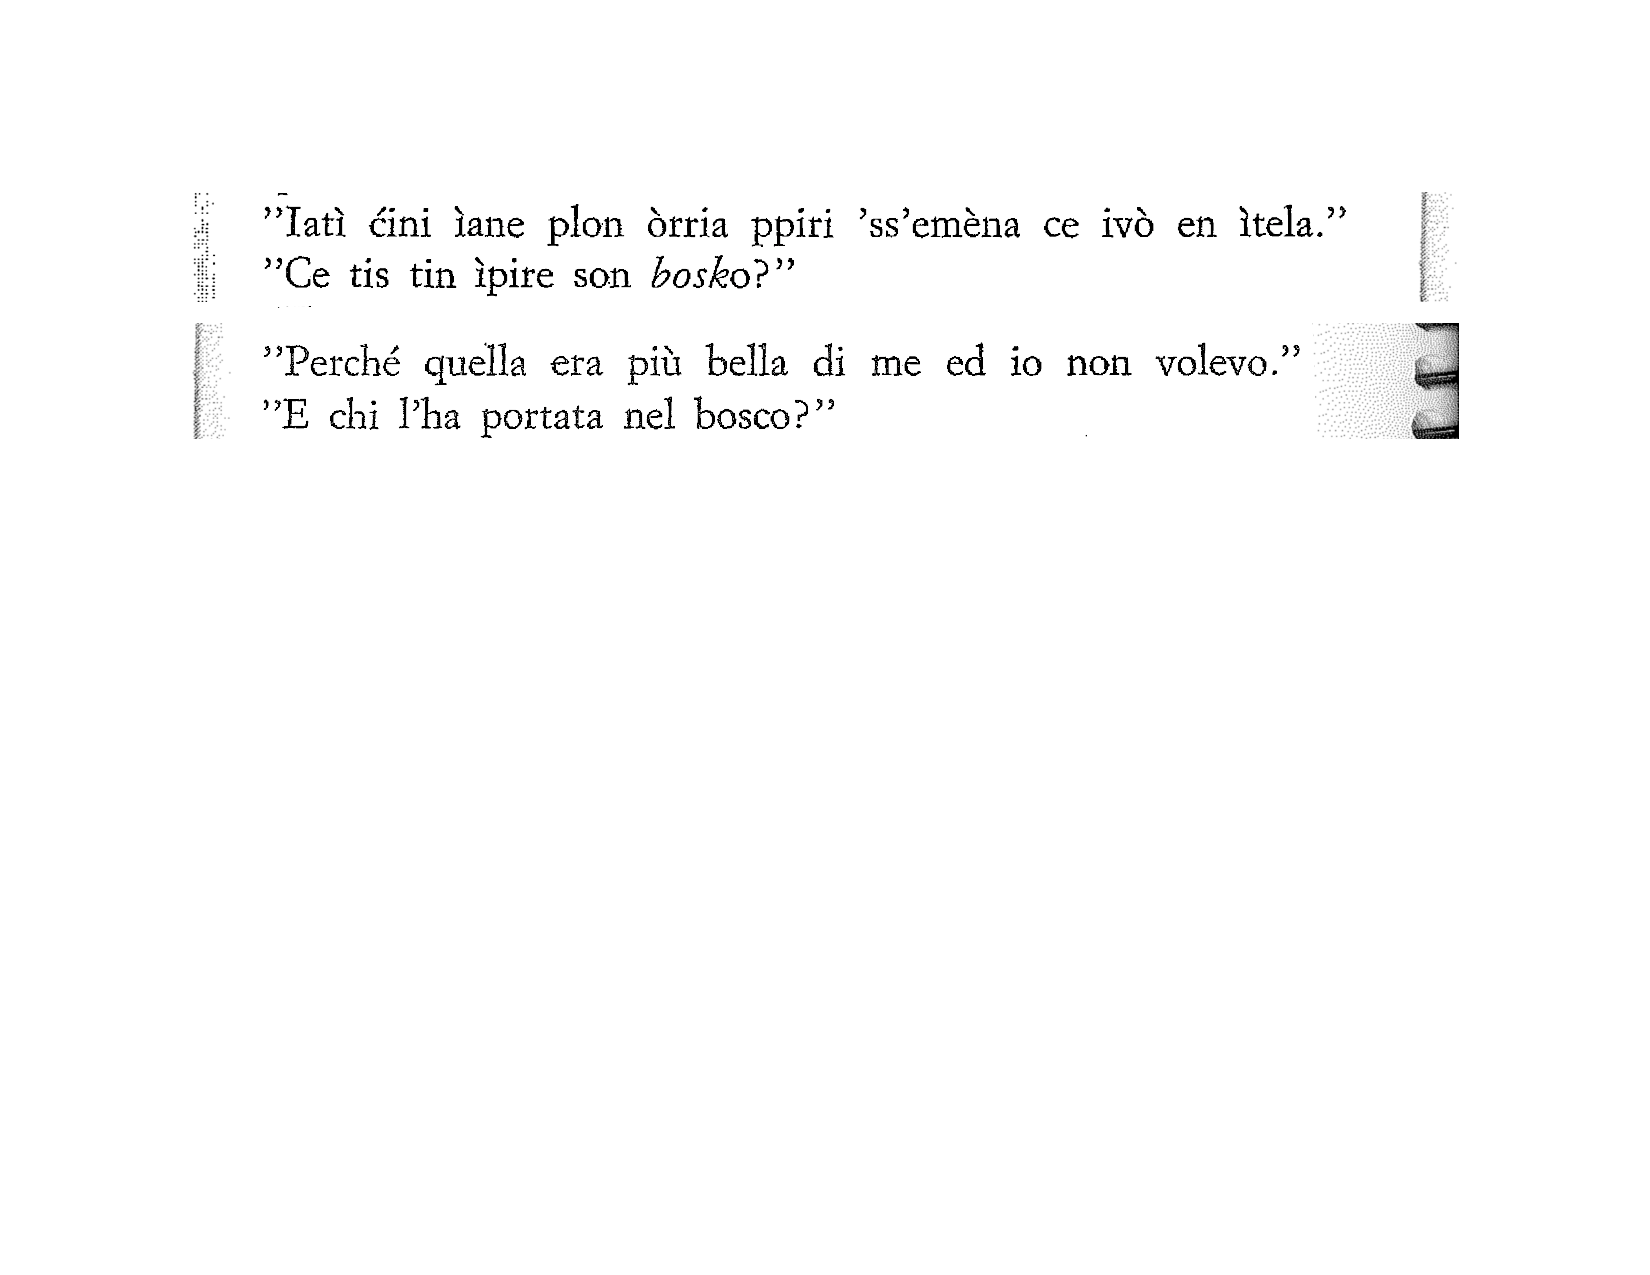
\includegraphics[width=0.93\columnwidth]{images/griko_example.pdf}}
      \vspace{0.7em}
    \end{subfigure}
    \begin{subfigure}[t]{\columnwidth}
      \centering
      \caption{Yakkha (top) -- Nepali (middle) -- English (bottom)}
      \vspace{-0.5em}
      \fbox{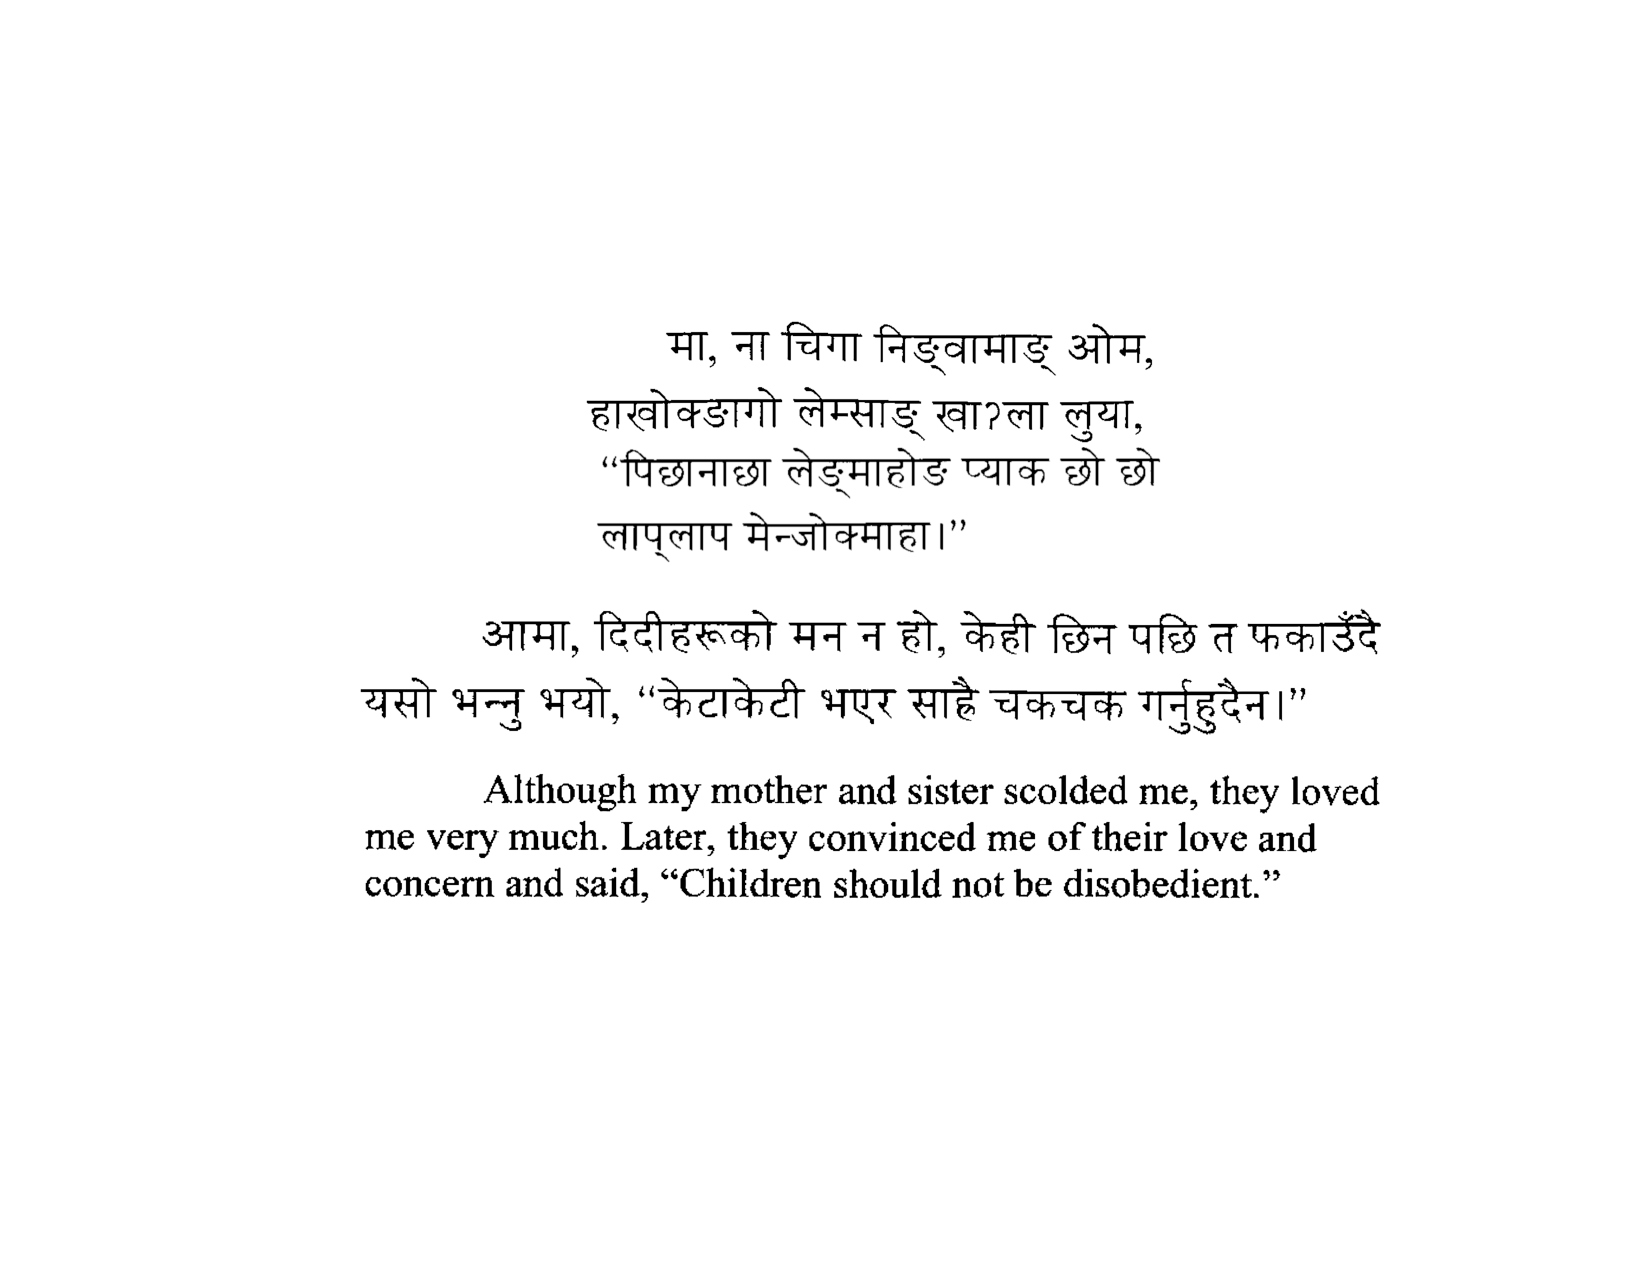
\includegraphics[width=0.9\columnwidth]{images/figure2c.pdf}}
      \vspace{0.6em}
    \end{subfigure}
    \footnotesize{(d) Handwritten Shangaji -- typed English glosses}
    \begin{tabular}{|@{\ \ }c@{\ \ }|}
    \hline
     \begin{subfigure}[t]{0.9\columnwidth}
      \centering
      
\includegraphics[width=0.9\columnwidth]{images/sha_img.pdf}
      
\includegraphics[width=0.5\columnwidth]{images/sha_text.pdf}
    \end{subfigure}\\
    \hline
    \end{tabular}
    \caption{Examples of scanned documents in endangered languages accompanied by translations from the same scanned book (a, b, c) or linguistic archive (d).}
    \label{fig:dataset_example}
    \vspace{-1.2em}
\end{figure}
